\section{V10}
\subsection{C/C++ Strukturen Umsetzen}
\subsubsection{Entscheidungen}
In Assembler-Sprache ist eine Entscheidung praktisch immer in einem 2-Stufigen Ablauf umgesetzt.
\begin{itemize}
    \item Benötigte Flags ermitteln
    \item Zugehörige bedingte Sprünge ausführen
\end{itemize}

Dabei wird nach folgendem Ablauf gearbeitet:\\
\vspace{-0.5cm}
\begin{enumerate}
    \item Vergleich: Zwei Werte werden subtrahiert, dabei wird nur auf die Flags geschaut.
    \item Anhand der Flags werden dann die bedingten Sprünge ausgeführt
\end{enumerate}

\subsubsection{Analyse von Hochsprachencode und Assembly-Code}
F"ur die Bestimmung der richtigen \textit{Conditional Branch} Instruktion kann wie am folgendem Beispiel gezeigt wird vorgegangen werden:

\begin{center}
	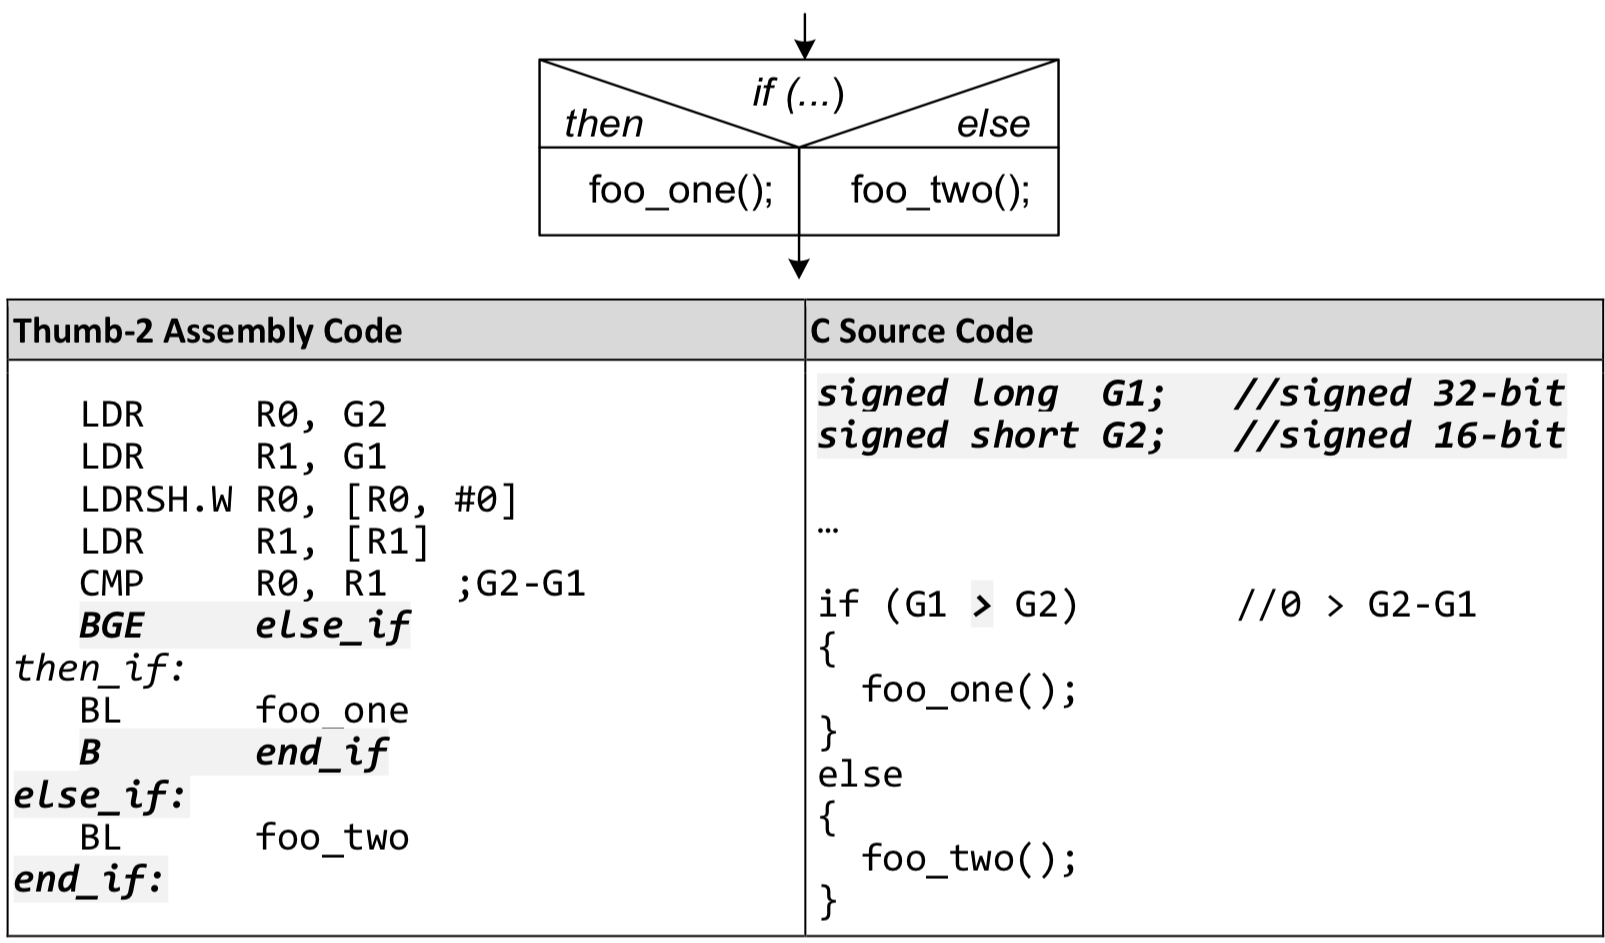
\includegraphics[width=10cm]{images/Bsp_cpp-assembly}
\end{center}

\begin{enumerate}
	\item Bestimmung des Datenformates der Variablen: \textit{signed} oder \textit{unsigned}\\
			$\Rightarrow$ Beispiel: signed
	\item Gleichung f"ur den \textit{Conditional Branch} aufstellen: \textbf{CMP Rn, Rm} entspricht Flags f"ur $Rn-Rm$\\
			$\Rightarrow$ Beispiel: $G1 > G2 \Leftrightarrow  0 > G2-G1$
\end{enumerate}
    
\begin{minipage}{9cm}
	\textbf{if-Block}\\
	F"ur einen Sprung in den if-Block w"are nun der Operator \color{red} \circled{$>$} \color{black} entscheidend.\\
	$\Rightarrow$ Conditional Branch Instruction: \textbf{BLT}\\
	Im Beispiel folgt jedoch der if-Block nach dem else-Sprung.
\end{minipage}
%
\begin{minipage}{0.5cm}
	\-\
\end{minipage}
%
\begin{minipage}{9cm}
	\textbf{else-if-Block}\\
	Die Gleichung wird zus"atzlich negiert:\\
	$0 > G2-G1$ = $\overline{0 \leq G2-G1}$\\
	F"ur einen Sprung in den else-if-Block w"are nun der Operator \color{red} \circled{$\leq$} \color{black} entscheidend.\\
	$\Rightarrow$ Conditional Branch Instruction: \textbf{BGE}
\end{minipage}

\subsubsection{Beispiele}
\begin{minipage}[t]{9cm}
	\textbf{IT-Instruktion}\\
	
	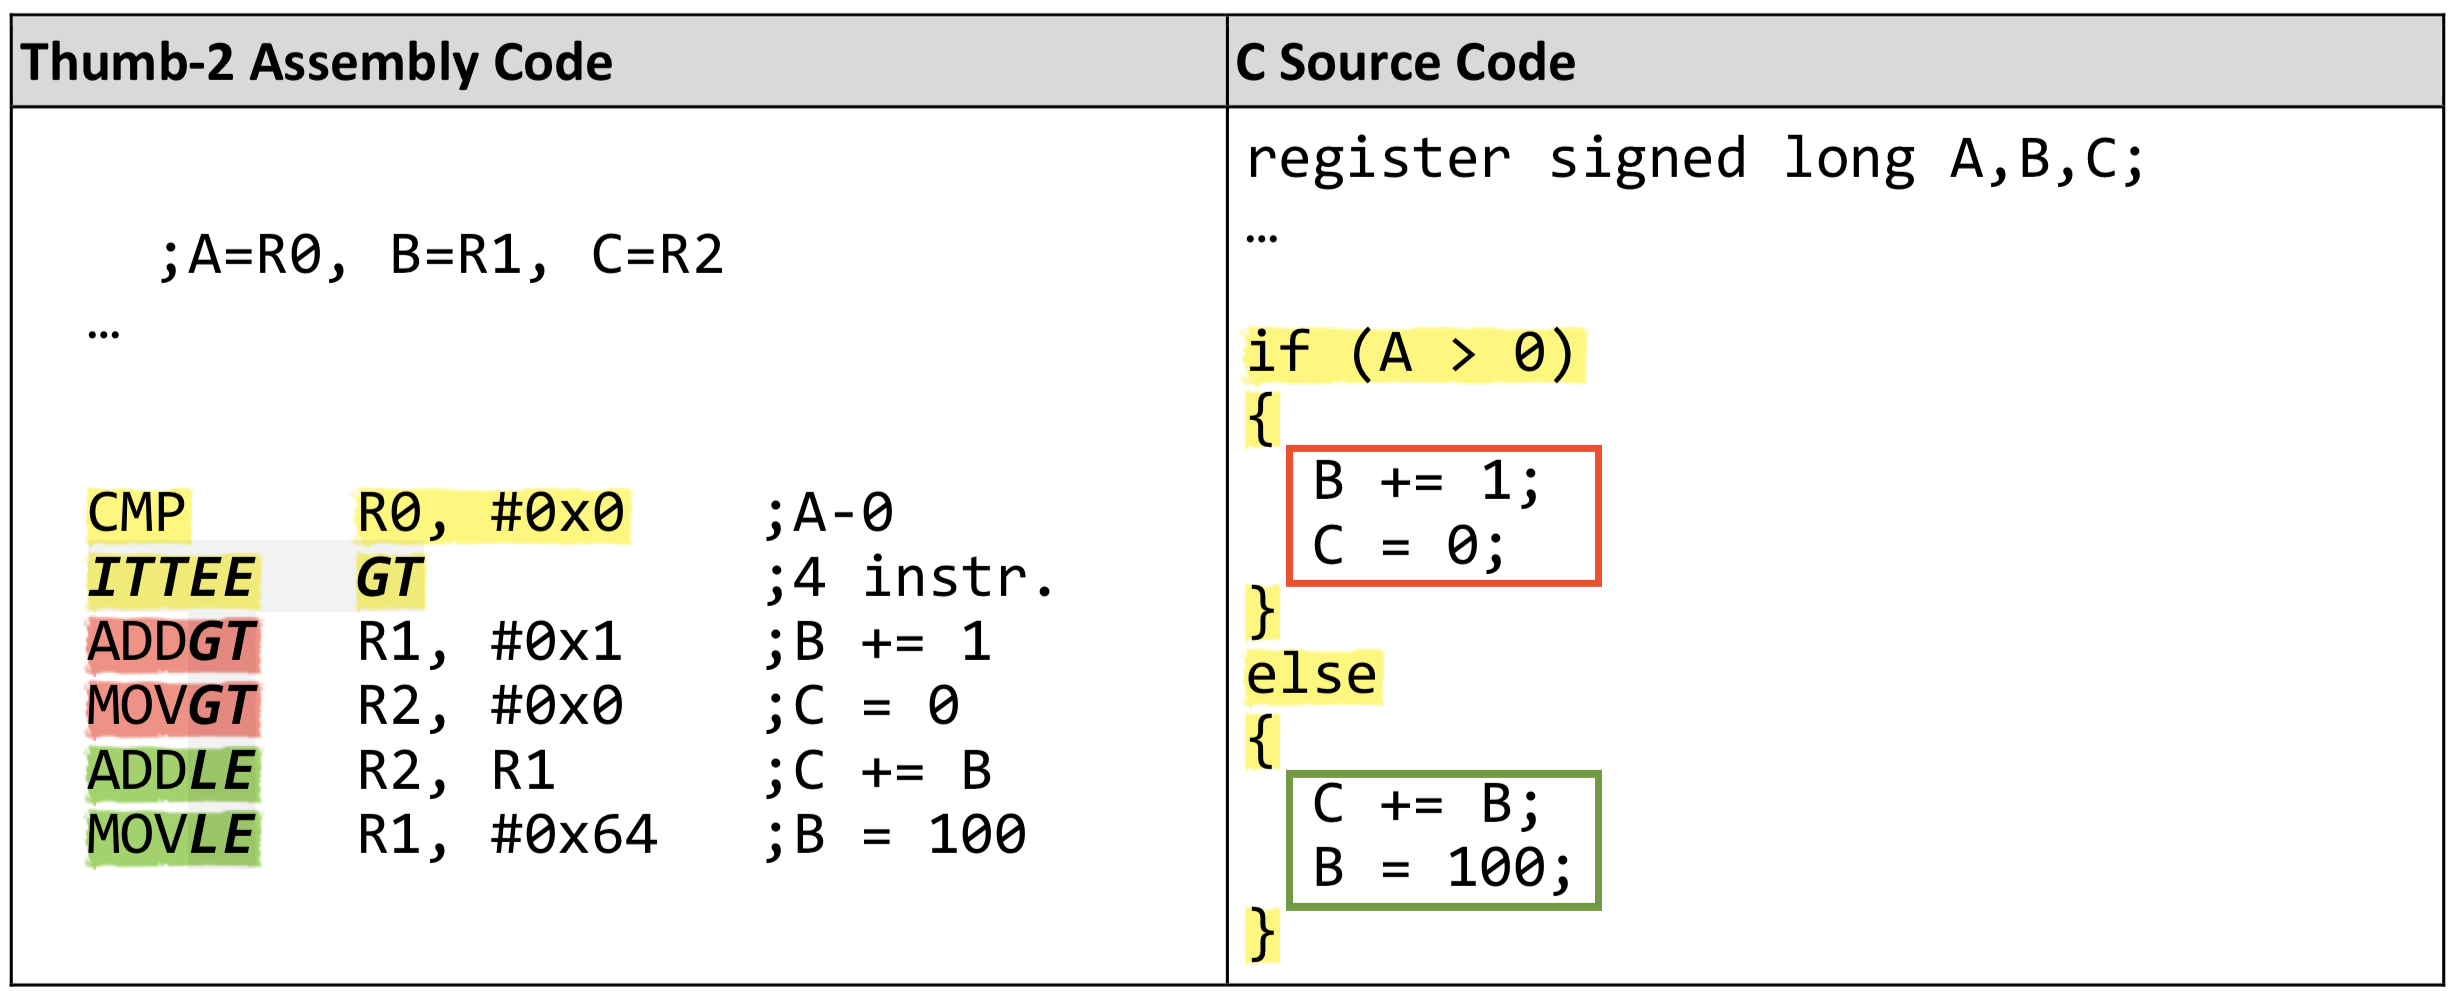
\includegraphics[width = 9cm]{images/IT-Instruction}
\end{minipage}
%
\begin{minipage}[t]{0.5cm}
	\-\
\end{minipage}
%
\begin{minipage}[t]{9cm}
	Wenn eine if..then..else Struktur nur wenige Sequenzen von Anweisungen enth"alt und keine \textit{Branches} kann dies auch mit der \textit{IT-Instruktion} umgesetzt werden, wobei diese maximal vier nachfolgende Anweisungen zu kontrollieren vermag.\\
	Die erste Instruktion im \textit{IT}-Block ist aktiviert, wenn der Condition-Code im Operandenfeld  erf"ullt ist. Die weiteren Anweisungen im Block werden durch anh"angen von eins bis drei Buchstaben mnemonisch gesteuert: T $\Rightarrow$ then; E $\Rightarrow$ else \\
		Allen Anweisungen im \textit{IT}-Block muss der entsprechende Condition-Code angeh"angt werden. Es werden \textbf{immer} gleich viele Taktzyklen ausgef"uhrt, egal welcher Pfad gefahren wird.
\end{minipage}
\newpage

\begin{minipage}[t]{9cm}
	\textbf{FOR-Schleife}\\
	
	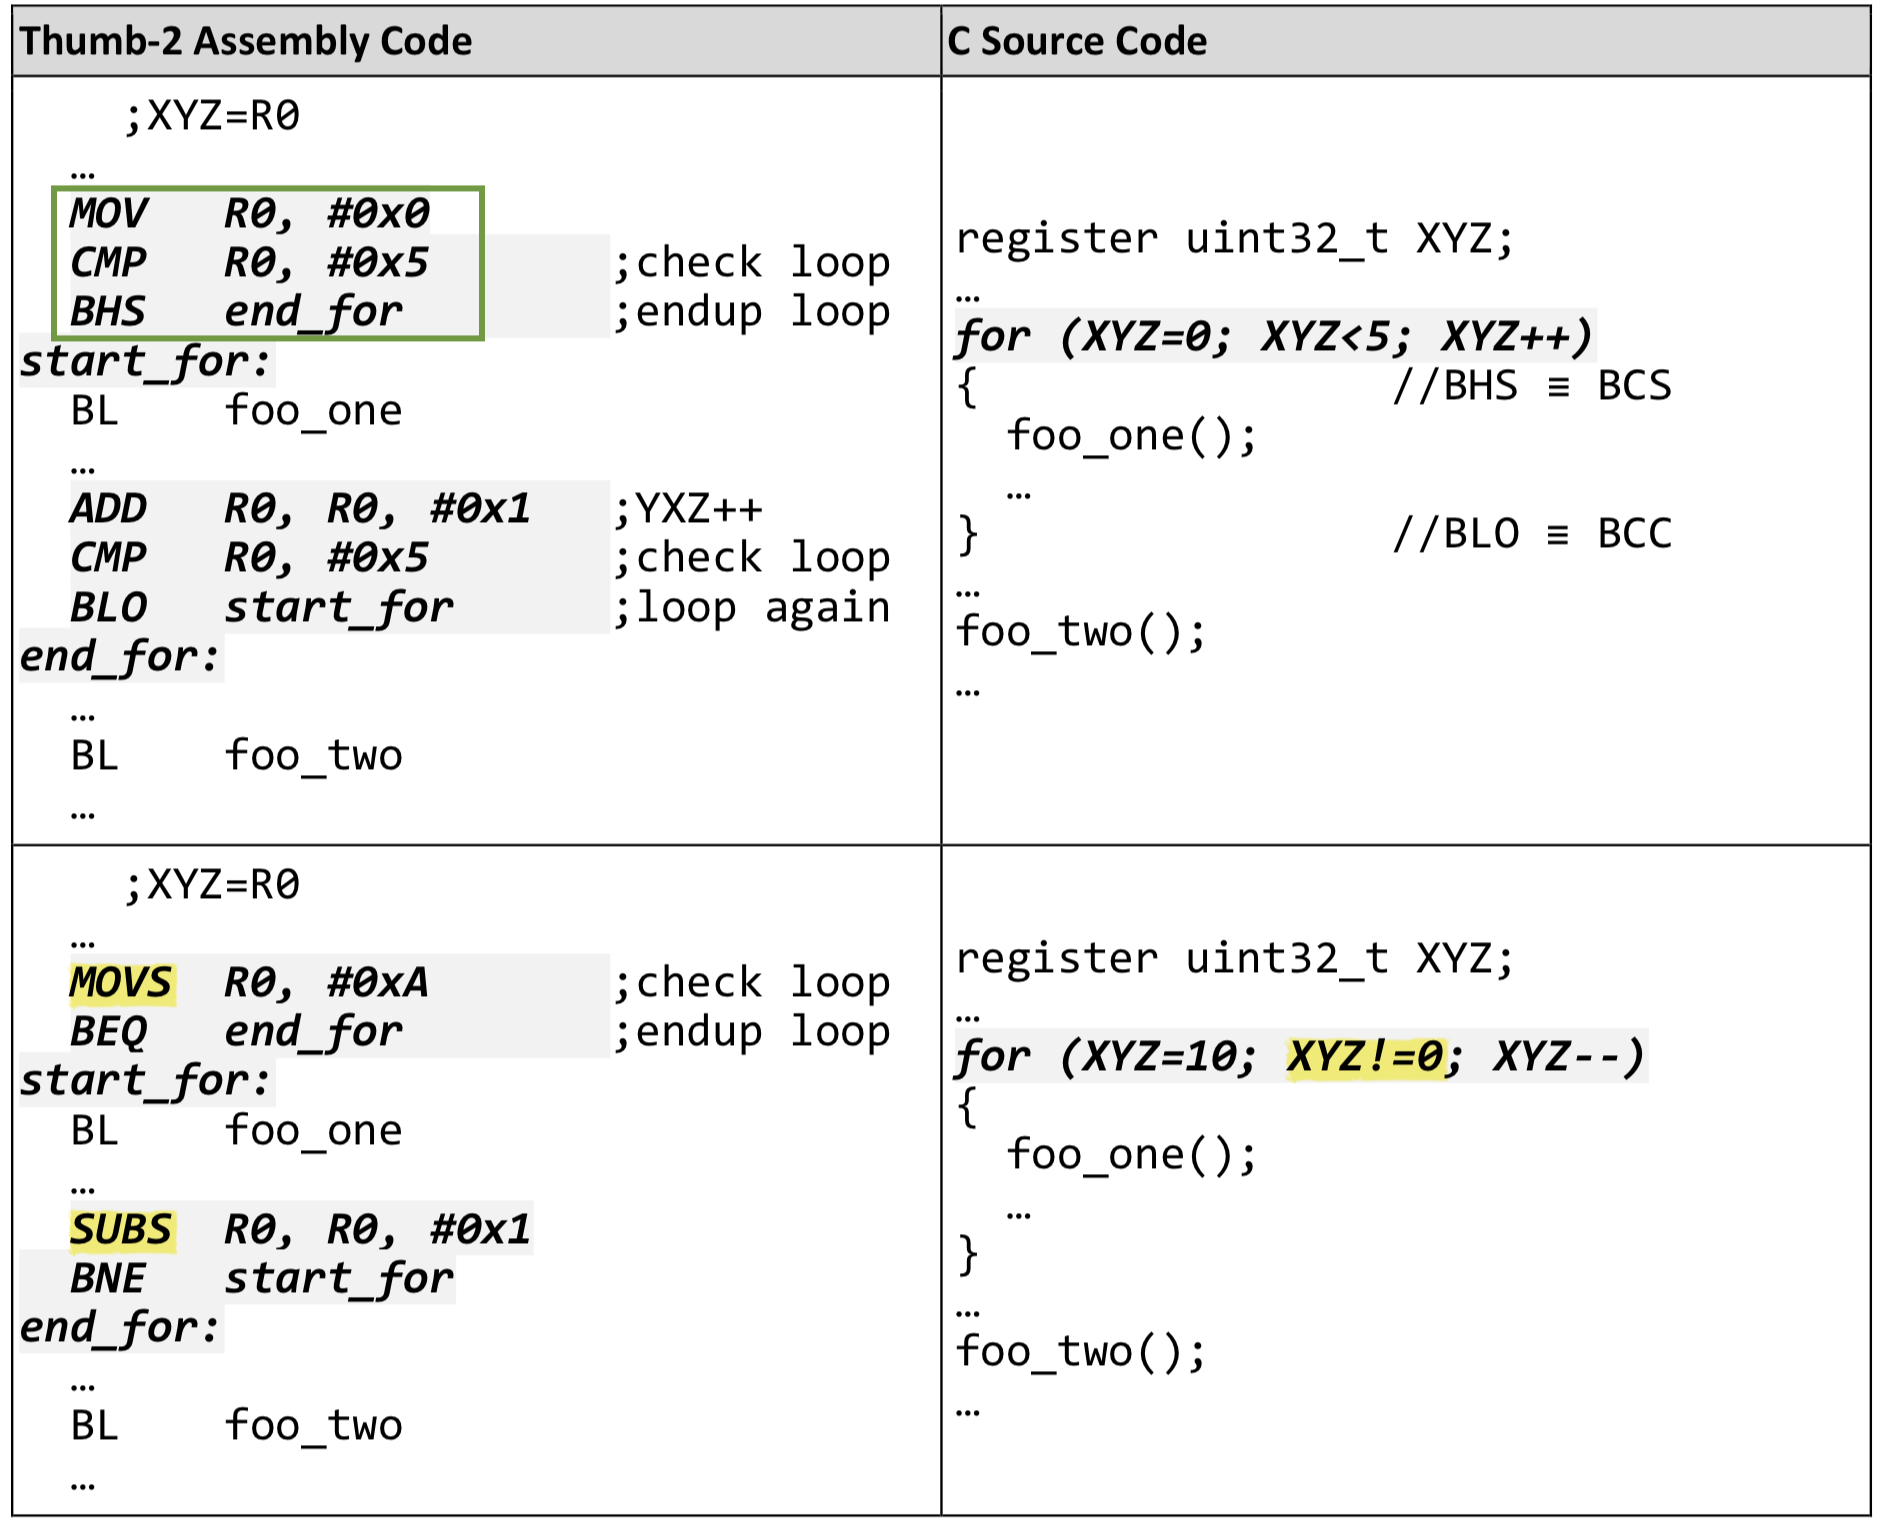
\includegraphics[width=9cm]{images/For-Loop}
\end{minipage}
%
\begin{minipage}[t]{0.5cm}
	\-\
\end{minipage}
%
\begin{minipage}[t]{9cm}
	Eine universelle Schleife (Iteration) besteht im Allgemeinen aus vier Teilen:
	\begin{itemize}
		\item Initialisierung \color{green} \tikz \draw (0,0) rectangle (0.6,0.3); \color{black}
		\item Test auf Abbruch oder Fortsetzung 
		\item Update der Loop-Control Variable
		\item Loop-Body (zu wiederholender Programm-Code)
	\end{itemize}
	
	Bei FOR-Schleifen, welche die Laufvariable gegen Null vergleichen, k"onnen so manche Instruktionen erspart werden. So k"onnen statt der \textit{CMP}-Instruktion die \colorbox{yellow}{\textit{MOVS-/SUBS}-Instruktionen} verwendet werden, welche gerade das \textit{Zero-Flag} evaluieren. Solange die Laufvariable nicht im Body verwendet wird, kann jede FOR-Schleife damit optimiert werden.
\end{minipage}

\newpage












